\documentclass[11pt]{article}
\usepackage{geometry}                % See geometry.pdf to learn the layout options. There are lots.
\geometry{a4paper}                   % ... or a4paper or a5paper or ... 
%\geometry{landscape}                % Activate for for rotated page geometry
%\usepackage[parfill]{parskip}    % Activate to begin paragraphs with an empty line rather than an indent
\usepackage{graphicx}
\usepackage{listings}		% for listings
\usepackage{booktabs}
\usepackage{multirow}
\usepackage{amssymb}
\usepackage{epstopdf}
\DeclareGraphicsRule{.tif}{png}{.png}{`convert #1 `dirname #1`/`basename #1 .tif`.png}
\usepackage{url}

\title{Embedded system, from software to hardware\\\small{(EDAN15 VT15 Final Report)}}
\author{
Anton Eliasson, \texttt{dat11ael@student.lu.se}\\
Daniel Lundell, \texttt{daniel.lundell.746@student.lu.se}
}
%\date{}                                           % Activate to display a given date or no date

\begin{document}
\lstset{
	language=C,
	captionpos=b,
	basicstyle=\footnotesize\ttfamily
}

\maketitle

\begin{abstract}
Brief description of the report. Context, hypothesis, experiments, results, conclusion. The abstract should contain enough
information about the rest of the document, but not too many details. Between 5--10 lines in this format.
\end{abstract}
\section{Introduction}
This is the lab report on the laboratory work in the Embedded Systems Design(EDAN15) course at LTH.


This is the part where you give background information and prepare the reader to deal with the rest of the document. \textit{This is the final report on the laboratory work in the Embedded Systems Design (EDAN15) course, LTH \ldots} Describe the lab work organization, its relation to the rest of the course as you see it.

\textit{The rest of the report is organized as follows. Section \ref{sec:exp} describes the experimental setup of each of the four labs. \ldots} Half a page for introduction will suffice.
\section{Experiments}\label{sec:exp}
The experiment was divided into 5 lab sessions. The goal was to evaluate software and harware solutions running on a Xilinix FPGA platform. The board used for testing was a Digilent Nexys-3.  

%Describe overall. Xilinx ISE Design Suite 14.x Digilent Nexys-3

First laboratory was to implement and compare two pure soft-ware solution of a Greatest Common Divisor (GCD) algorithm for N numbers. Furthermore, the software has to run on a single processor system.

Second laboratory session was to implement and evaluate again a pure software solution of a gcd algorithm for N numbers. This time the architecture should use a multi-processor system. The system uses two MicroBlaze processors, working on the same data set.

Third and fourth  laboratory session was to choose a part of the gcd algorithm for N number and implement it in hardware. The hardware part was writen and simulated in VHDL using Xilinx ISE.  The hardware should input/output data following a protocol specifed in the laboratory manual.

Last laboratory session was to integrate the hardware developed in the previous session into a larger system. The system should contain software to write the necessary communication and computations, to obtain a functioning hardware/software solution for the gcd of N-numbers problem.

%Describe what you have to do as laboratory work. Describe your application, target platform. Give information about the host platform and tool chain. Use references (here and whenever appropriate elsewhere in the report) to publications \cite{microblaze} or web pages (e.g. for companies \cite{xilinx}). Do avoid giving random web pages and wikipedia as reliable sources of information.
\subsection{Software algorithms}
The software algorithm choosen was the Euclidean subtraction algorithm. This was choosen to avoid the need of calculations using division, modulo and recursion. The algorithm is very simple and well defined. 
\begin{lstlisting}[float=tbh,frame=tb,captionpos=b,caption={Working on your report},label=lst:example]
function gcd(a,b)
	while(a != b) {
		if a>b
			a = a-b
		else
			b = b-a
	}
	return a;
}
\end{lstlisting}

\subsection{Single processor}
Describe what is particular to this solution.
\subsection{Dual processor}
The dual processor system was implemented using two separate MicroBlaze cores. The communicated using two FSL-connections connected to each core. This was choosen over sharing memory between the two cores. Relation between the cores was divided into master/slave where one core acted as the master. The software was divided onto the two cores accordingly with the master/slave principle. Software on the master core was responsible for fetching the input data, split it and send half of it to the slave core. The slave core contained only the code for communcating through FSL and calculating gcd. The master and slave core calculated gcd for their share of the data and. Final caluclation was done on the master core after the slave had returned the gcd for the data set on the slave core.
%Describe what is specific to this solution. How do you divide the work between the processors? How do you communicate in between them? Are there any other ways to do this? How did you make sure your solution works properly? How did you test it? Debug it in any way?
\subsection{Hardware accelerated}
Describe your specific hardware accelerator. Describe the structure and behavior. Why did you choose to implement exactly this part of the algorithm? How does it fit in the whole system? How did you make sure your solution works properly? How did you test it? Debug it in any way?

Use pictures and timing diagrams, such as the one in Figure \ref{fig:example}. Do explain every picture and diagram.

\begin{figure}[!htb]
   \centering
   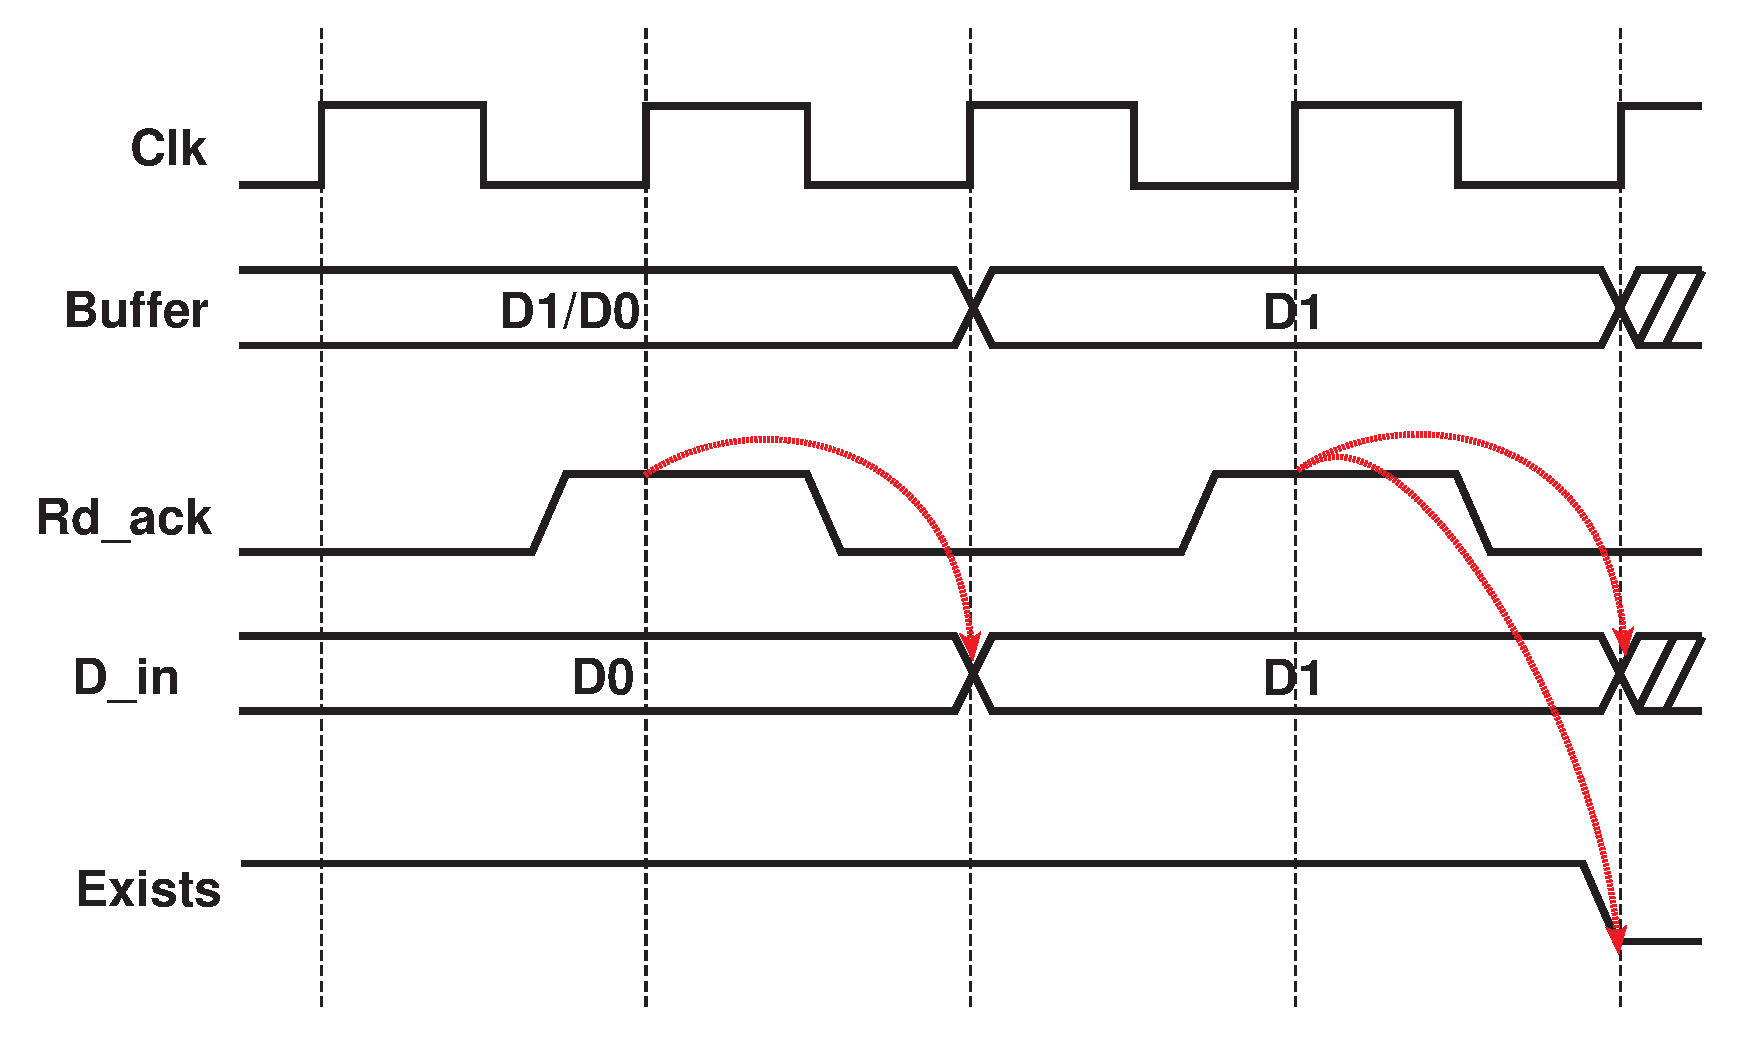
\includegraphics[width=0.6\textwidth]{example} 
   \caption{A figure example}
   \label{fig:example}
\end{figure}

\section{Measurements and Discussion}
This is probably the most important part of the report. In here you must describe the what and how you measure. Describe any specific parts in the hardware architecture or the software that help you conduct measurements. You should use graphs or tables to present your results, such as Table \ref{tab:example} or \ref{tab:example2}, but do not forget to describe the measures and units in the columns or graph axis.

% Requires the booktabs if the memoir class is not being used
\begin{table}[htbp]
   \centering
   %\topcaption{Table captions are better up top} % requires the topcapt package
   \begin{tabular}{@{} lcr @{}} % Column formatting, @{} suppresses leading/trailing space
      \toprule
      \multicolumn{2}{c}{Item} \\
      \cmidrule(r){1-2} % Partial rule. (r) trims the line a little bit on the right; (l) & (lr) also possible
      Animal    & Description & Price (\$)\\
      \midrule
      Gnat      & per gram & 13.65 \\
                & each     &  0.01 \\
      Gnu       & stuffed  & 92.50 \\
      Emu       & stuffed  & 33.33 \\
      Armadillo & frozen   &  8.99 \\
      \bottomrule
   \end{tabular}
   \caption{Avoid vertical lines in tables.}
   \label{tab:example}
\end{table}

\begin{table}[htbp]
   \centering 
 \begin{tabular}{cc|c|c|c|c|l}
\cline{3-6}
& & \multicolumn{4}{|c|}{Primes} \\ \cline{3-6}
& & 2 & 3 & 5 & 7 \\ \cline{1-6}
\multicolumn{1}{|c|}{\multirow{2}{*}{Powers}} &
\multicolumn{1}{|c|}{504} & 3 & 2 & 0 & 1 &     \\ \cline{2-6}
\multicolumn{1}{|c|}{}                        &
\multicolumn{1}{|c|}{540} & 2 & 3 & 1 & 0 &     \\ \cline{1-6}
\multicolumn{1}{|c|}{\multirow{2}{*}{Powers}} &
\multicolumn{1}{|c|}{gcd} & 2 & 2 & 0 & 0 & min \\ \cline{2-6}
\multicolumn{1}{|c|}{}                        &
\multicolumn{1}{|c|}{lcm} & 3 & 3 & 1 & 1 & max \\ \cline{1-6}
\end{tabular}
  \caption{Uses \textit{multirow} \LaTeX package}
   \label{tab:example2}
\end{table}
Say a few words about the complexity of the different solutions and how long did it take to reach a working design.
 
\subsection{Performance}
Give the performance figures for your solutions. Note that both the number of clock cycles \textsc{and} the clock frequency is important for performance! 

Discuss how and why the figures are different in between solutions. Discuss how these figures are different from your expectation. For example, should a dual processor system be twice faster than a single processor system? Is it? Why?
How about compiler optimizations? 

Explain whether and how the data sets your algorithm operates on influence the results. For example, why computing the something for 10 numbers is slower than computing the same thing for 30 numbers?

\subsection{Device Utilization}
Give the FPGA resources consumed by each of your solutions. Explain how these relate to each other -- e.g. whether a dual processor system has double the area of a single processor system and how do these relate to the hardware accelerated solution. Explain why or how using different algorithms influences or not the device utilization.

\subsection{Power and Energy}
The power and energy consumption are also important for a design. The XPower Analyser that comes with the Xilinx ISE helps you determine the power consumption for your designs. Have a look at the hierarchical breakdown of power consumption and identify the parts of your design that consume a lot of power. Also, as you know energy is the time integral of power:
\begin{equation}
E = \int_{t_1}^{t_2} P dt \approx P \Delta t
\end{equation}
How do your different solutions compare from the power and energy consumption point of view?

\section{Summary}
In this part you briefly summarize your report. Continue with conclusions, lessons learned, unexpected results, unsolved problems or other issues that remain open. Relate back to the content of the course and explain whether or how the laboratory work helped you or not with understanding certain issues from the theoretical part.

\bibliographystyle{plain}
\bibliography{abibfile}

\end{document}  
